\documentclass[main.tex]{subfiles}

%\usepackage[]{algorithm2e}

\usepackage{algorithmicx}
\usepackage[Algorithm,ruled]{algorithm}
\usepackage{algorithm,algcompatible,amsmath}
\algnewcommand\DESCRIPTION{\item[\textbf{Opis:}]}%
\algnewcommand\INPUT{\item[\textbf{Ulaz:}]}%
\algnewcommand\OUTPUT{\item[\textbf{Izlaz:}]}%

\algnewcommand\algorithmicforeach{\textbf{for each}}
\algdef{S}[FOR]{ForEach}[1]{\algorithmicforeach\ #1\ \algorithmicdo}

\usepackage{mathtools}

\begin{document}

Metoda promenljivih okolina (VNS, eng. \textit{Variable Neighbourhood Search}) je \\ S-metaheuristika (\textit{Single-solution-based} metaheuristika) zasnovana na lokalnoj pretrazi i unapređivanju jednog rešenja, za razliku od genetskog algoritma koji istovremeno radi nad velikim brojem rešenja. Lokalna pretraga polazi od početnog rešenja i u njegovoj okolini pokušava da pronađe bolje rešenje. Zatim se postupak pretrage nastavlja od tog rešenja, i ponavlja se sve dok se ne pronađe bolje rešenje. VNS metaheuristika je prvobitno predložena za rešavanje problema trgovačkog putnika u radu \cite{vnsFirstPaper} koji su objavili Pjer Hansen i Nenad Mladenović. Metoda promenljivih okolina zasnovana je na tri činjenice:

\begin{enumerate}
  \item Lokalni optimum u odnosu na jednu okolinu ne mora da predstavlja lokalni optimum u odnosu na drugu.
  \item Globalni optimum je lokalni optimum u odnosu na sve moguće okoline.
  \item Za mnoge probleme lokalni optimumi u odnosu na različite okoline su relativno blizu.
\end{enumerate}

Poslednja činjenica ukazuje na to da lokalni optimum često daje neke informacije o globalnom. Zato se okoline lokalnog optimuma istražuju u potrazi za boljim rešenjem u nadi da će pretraga dovesti do globalnog optimuma \cite{vnsHandbook}.

Osnovnu varijantu metode promenljivih okolina (Basic VNS, eng. \textit{Basic Variable Neighbourhood Search}) čine lokalna pretraga i stohastička procedura razmrdavanja (eng. \textit{shaking}). Cilj ove procedura je da spreči da se pretraga zaglavi u nekom lokalnom optimumu. Osnovni koraci ove metode su:

\begin{enumerate}
  \item Inicijalizacija: Izbor skupa okolina $N_k, k = 1, ..., k_{max}$; Konstruisanje početnog rešenja x; Izbor kriterijuma zaustavljanja.
  \item Ponavljanje narednih koraka sve dok se ne ispuni kriterijum zaustavljanja:
  \begin{enumerate}
    \item Postaviti k = 1
    \item Ponavljati naredne korake sve dok je $k \leq k_{max}$
        \begin{enumerate}
        \item \textit{Razmrdavanje} - Generisanje slučajnog rešenja $x'$ iz okoline $N_k(x)$ ;
        \item \textit{Lokalna pretraga} - Primeniti neku metodu lokalne pretrage sa početnim rešenjem $x'$. Rezultat pretrage označiti sa $x''$;
        \item \textit{Prihvatanje rešenja i promena okoline} - Ako je tako dobijeno rešenje $x''$ bolje od  $x$, postaviti $x$ = $x''$ i  $k = 1$; Inače, postaviti $k = k + 1$;
      \end{enumerate}
  \end{enumerate}
\end{enumerate}


Kako su kod simboličke regresije rešenja predstavljena pomoću stabala, svaki od ovih koraka je bilo potrebno definisati u skladu sa takvim strukturama podataka. U radu \cite{vnp} je predložena osnovna VNP (eng. \textit{Basic Variable Neighbourhood Programming}) metoda koja je usklađena sa svim zahtevima simboličke regresije.


\subsection{Tipovi okolina}
\label{sec:neighbourhoodStructure}

Kod osnovne VNP metode se koriste tri vrste okolina:

\begin{itemize}
    \item $N(T)$ označava strukturu susedstva koje se koristi tokom lokalne pretrage. Članovi ove vrste susedstva se formiraju elementarnim transformacijama stabla, koje će biti predstavljene nešto kasnije. %opisane u narednim sekcijama. 
    
    \item $N_1(T)$ označava strukturu susedstva čiji se članovi dobijaju zamenom samo jednog čvora početnog stabla $T$. Čvorovi koji predstavljaju funkcije se mogu zameniti samo čvrovima koji predstavljaju funkcije iste arnosti. Slično, terminali se mogu zameniti samo terminalima. Dobijeni susedi imaju isti oblik i veličinu kao stablo $T$. Ovaj operator odgovara operatoru mutacije pojedinačnog čvora (eng. \textit{point mutation}) kod genetskog programiranja.
    
    Na primer, ako $T$ predstavlja izraz $ \max \left\{\frac{3}{x_{3} * 2.4} ; x_{1}-x_{2}\right\} $, a skupovi funkcija i terminala redom sadrže $\{*, -, +\}$ i $\{3, 2.4, 0.66, x1, x2, x3, x4\}$, onda su neki od suseda stabla $T$: $\max \left\{\frac{2.4}{x_{3} * 2.4} ; x_{1}-x_{2}\right\}$, $\max \left\{\frac{x_{1}}{x_{3} * 2.4} ; x_{1}-x_{2}\right\}$, $\max \left\{3 + x_{3} * 2.4 ; x_{1}-x_{2}\right\}$, itd.
    
    \item $N_2(T)$ predstavlja operator zamene (eng. \textit{Swap operator}). U ovoj okolini, susedi od $T$ se generišu tako što se u $T$ nasumično odabre jedan čvor koji predstavlja koren podstabla koje treba da bude zamenjeno. Na njegovo mesto se postavlja novo, slučajno generisano stablo. Oblik i veličina generisanog suseda se razlikuju od početnog stabla $T$. Pomoću ovog operatora može se generisati beskonačan broj suseda. \textit{Swap operator} odgovara operatoru mutacije celog podstabla (eng. \textit{subtree mutation}) kod genetskog programiranja.
    
    Okoline $N_1(T)$ i $N_2(T)$ se koriste u proceduri razmrdavanja.
\end{itemize}


\subsection{Razmrdavanje}
\label{sec:shaking}

Procedura razmrdavanja je prikazana u algoritmu \autoref{alg:shaking}. Ovom procedurom se dobija $k$-ti sused stabla $T$, primenom istog poteza $k$ puta. Odnosno, prvo je potrebno nasumično izabrati okolinu $N_1(T)$ ili $N_2(T)$, a zatim taj operator primeniti $k$ puta nad datim stablom.

\begin{algorithm}
\floatname{algorithm}{Algoritam}
\caption{Shake(T, k)}
\label{alg:shaking}
  \begin{algorithmic}[1]
    \INPUT $T$ - inicijalno stablo, k - broj ponavljanja primene operatora susedstva;
    \OUTPUT $T'$ - stablo koje je sused stabla $T$;
    \STATE $s \leftarrow$ slučajna vrednost iz $\{1,2\}$;
    \FOR {$i = 1,k$}
        \STATE Na slučajan način izabrati $T' \in N_s(T)$ ;
        \STATE $T \leftarrow T'$;
    \ENDFOR
    \STATE \textbf{return} T;
  \end{algorithmic}
\end{algorithm}

\subsection{Elementarne transformacije i lokalna pretraga}
\label{sec:ETT}

Susedi koji se razmatraju tokom lokalne pretrage, generišu se elementarnim transformacijama trenutno najboljeg rešenja.

Elementarne transformacije stabla (ETT, eng. \textit{Elementary Tree Transformation}) se definišu na sledeći način. Neka je $G(V, E)$ neusmereni graf sa skupom čvorova $V$ i skupom grana $E$ i neka je $T(V, A)$ neko razapinjuće stablo grafa $G$. ETT transformiše stablo $T$ u stablo $T'$ (u oznaci $T' = ETT(T)$) sledećim koracima:

\begin{enumerate}
    \item U stablo $T$ dodati granu $a$, takvu da $a \in E \setminus A$.
    \item Detektovati formirani ciklus i ukloniti bilo koju granu (osim one koja je dodata u prethodnom koraku) iz njega kako bi se dobio podgraf $T'$, koji takođe predstavlja razapinjuće stablo grafa $G$.
\end{enumerate}

Ovaj postupak je opisan algoritmom \autoref{alg:ETT}. Ulazni parametar je stablo $T(r, F, H, E, d)$, definisano korenom $r$, skupom čvorova koji predstavljaju funkcije $F$, skupom čvorova koji predstavljaju terminale $H$, skupom grana $E$ i nizom $d = (d_1, ..., d_n)$ koji označava stepen svakog čvora stabla $T$. Stepen $d_i$ označava broj grana koje su incidentne sa čvorom $i$. Ako čvor predstavlja binarnu funkciju, njegov stepen je 3, a ako predstavlja unarnu funkciju, njegov stepen je 2. Stepen čvora terminala je 1.

\begin{algorithm}
\floatname{algorithm}{Algoritam}
\caption{ETT(T(r, F, H, E, d))}
\label{alg:ETT}
  \begin{algorithmic}[1]
    \STATE $Terminate \leftarrow false$; 
    \ForEach {node $i \in F $}
        \ForEach {node $j \in F \cup H \setminus \{i, parent(i), child(i)\} $}
            \STATE $E^{\prime} \leftarrow E \cup\{(i, j)\}$; \color{gray} // ciklus je formiran \color{black}
            \STATE $d_{i} \leftarrow d_{i}+1 ; d_{j} \leftarrow d_{j}+1$;
            \IF{$j \in F $}
                \STATE \color{gray}// slučaj 1 \color{black}
                \STATE $E^{\prime} \leftarrow E^{\prime} \backslash\{(x, b)\} / x \in\{i, j\}, b \in\{\text {parent}(i), \text{parent}(j)\}$;
                \STATE $d_{b} \leftarrow d_{b}-1$ ;
                \IF{$x = i$}
                    \STATE $d_{i} \leftarrow d_{i}-1 ; E^{\prime} \leftarrow E^{\prime} \cup\{(b, \operatorname{child}(j))\}$;
                    \STATE $d_{b} \leftarrow d_{b}+1 ; d_{\text {child}(j)} \leftarrow d_{\text {child}(j)}+1$;
                    \STATE $E^{\prime} \leftarrow E^{\prime} \backslash\{(j, \text { child}(j))\}$;
                    \STATE $d_{j} \leftarrow d_{j}-1 ; d_{\text {child}(j)} \leftarrow d_{\text {child}(j)}-1$;
                \ELSE
                    \STATE $d_{j} \leftarrow d_{j}-1 ; E^{\prime} \leftarrow E^{\prime} \cup\{(b, \text { child}(i))\}$;
                    \STATE $d_{b} \leftarrow d_{b}+1 ; d_{child}(i) \leftarrow d_{\text {child}(i)}+1$;
                    \STATE $E^{\prime} \leftarrow E^{\prime} \backslash\{(i, \text { child}(i))\}$;
                    \STATE $d_{i} \leftarrow d_{i}-1 ; d_{\text {child}(i)} \leftarrow d_{\text {child}(i)}-1$;
                \ENDIF
            \ELSE 
                \STATE \color{gray}// slučaj 2 \color{black}
                \STATE $b \leftarrow \operatorname{parent}(j) ; E \leftarrow E^{\prime} \backslash\{(j, b)\}$;
                \STATE $d_{j} \leftarrow d_{j}-1 ; d_{b} \leftarrow d_{b}-1$;
                \STATE $E^{\prime} \leftarrow E^{\prime} \cup\{(b, c h i l d(i))\}$;
                \STATE $d_{b} \leftarrow d_{b}+1 ; d_{\text {child}(i)} \leftarrow d_{\text {child}(i)}+1$;
                \STATE $E^{\prime} \leftarrow E^{\prime} \backslash\{(i, \text { child }(i))\}$;
                \STATE $d_{i} \leftarrow d_{i}-1 ; d_{\text {child}(i)} \leftarrow d_{\text {child}(i)}-1$;
             \ENDIF
             \STATE $T^{\prime} \leftarrow T\left(r, F, H, E^{\prime}, d\right)$;
             \IF{$f\left(T\left(r, F, H, E^{\prime}, d\right)\right)>f(T(r, F, H, E, d))$}
                \STATE $E \leftarrow E^{\prime} ; \text { $Terminate$ } \leftarrow \text { $true$}; \text { Break; }$
             \ENDIF
        \ENDFOR
        \IF{$Terminate = true$}
            \STATE \text { Break; }
        \ENDIF
    \ENDFOR
  \end{algorithmic}
\end{algorithm}

Naredbe iz algoritma \autoref{alg:ETT} se mogu grupisati u četiri grupe (dve vrste dodavanja grane i dve vrste uklanjanja grane):

\begin{enumerate}
    \item \textit{Dodavanje grane (tip I)} (linije 4,5). Grana $(i,j)$ se dodaje u trenutno stablo $T$, pri čemu ni $i$ ni $j$ ne smeju biti koren stabla. Dodatno, ili $i$ ili $j$ mora da bude funkcija. Nakon primene ovog koraka se formira ciklus u trenutnom stablu.
    \item \textit{Uklanjanje grane (tip I)} (linije 8,9,23,24). Ovde postoje dva slučaja. Ako su i $i$ i $j$ funkcije (slučaj 1 u algoritmu), onda se može ukloniti neka od grana $(i, parent(i))$, $(j, parent(j))$ kako bi se uklonio ciklus. Ako je jedan od čvorova terminal, npr. neka to bude $j$, onda se uklanja grana $(j, parent(j))$ (slučaj 2 u algoritmu).
    \item \textit{Dodavanje grane (tip II)} (linije 11,12,16,17,25,26). Ako je obrisana grana $(i, parent(i))$, onda se dodaje grana $(parent(i), child(j))$. Ako je obrisana grana $(j, parent(j))$, onda se dodaje grana $(parent(j), child(i))$. 
    \item \textit{Uklanjanje grane (tip II)} (linije 13,14,18,19,27,28). Ove grane se uklanjaju kako bi stepen čvorova ostao zadovoljavajući.
\end{enumerate}

Na slici \ref{fig:ett} je prikazan primer formiranja jednog suseda stabla sa slike \ref{fig:syntaxTree} pomoću elementarnih transformacija. Koraci algoritma \autoref{alg:ETT} na ovom primeru bi bili sledeći:
\begin{itemize}
    \item $Terminate = false$
    \item $i \in F = \{-,/,*\}$: Npr. uzima se da je $i = {}'-'$. Kako je stepen funkcijskih čvorova jednak 3, važi $d_i = 3$.
    \item $j \in F \cup H \setminus \{i, parent(i), child(i)\}$: Npr. $j = {}'*', d_j = 3$
    \item $E^{\prime} \leftarrow E \cup\{(i, j)\}$: U trenutno stablo se dodaje grana $({}'-', {}'*')$ (Slika \ref{fig:ett}, korak 2). Time se dobija ciklus koji povezuje čvorove ${}'-', {}'*', {}'/', {}'max'$. Ovde se, takođe, povećavaju stepeni čvorova ${}'-'$ i ${}'*'$. Sada važi $d_i = 4$ i $d_j = 4$.
    \item Kako je odabano $j = {}'*'$, znači da $j \in F$, što znači da se izvršava prvi slučaj algoritma.
    \item $E^{\prime} \leftarrow E^{\prime} \backslash\{(x, b)\} / x \in\{i, j\}, b \in\{\text {parent}(i), \text{parent}(j)\}$: Ovde se može obrisati grana $(i, parent(i))$, što je $({}'-', {}'max')$, ili grana $(j, parent(j))$, što je $({}'*', {}'/')$. Odabraće se npr. grana $({}'*', {}'/')$ (Slika \ref{fig:ett}, korak 3). Znači, $x = j$ i $b = parent(j)$, pa se dalje izvršava blok koda od 16. do 19. linije.
    \item Smanjuje se stepen čvorova $j$ i $parent(j)$: $d_j = 3$, $d_{parent(j)} = 2$ (Slika \ref{fig:ett}, korak 4).
    \item $E^{\prime} \leftarrow E^{\prime} \cup\{(b, \text { child}(i))\}$: Sada se dodaje grana $(parent(j), child(i))$, što može biti $({}'/', {}'x_1')$ ili $({}'/', {}'x_2')$. Neka je npr. odabrana $({}'/', 'x_1')$ (Slika \ref{fig:ett}, korak 5).
    \item Sada se povećava stepen čvora $child(i)$, što je ${}'x_1'$, i čvora $parent(j)$, što je ${}'/'$: $d_{parent(j)} = 3$, $d_{child(i)} = 2$.
    \item $E^{\prime} \leftarrow E^{\prime} \backslash\{(i, \text { child}(i))\}$: Konačno, briše se grana $({}'-', {}'x_1')$ i ažuriraju se stepeni $d_i = 3$ i $d_{child(i)} = 1$ (Slika \ref{fig:ett}, korak 6). Primećujemo da novo stablo $T(r, F, H, E{}', d)$ čuva stepen svakog čvora iz originalnog stabla $T(r, F, H, E, d)$.
    \item Ako je funkcija prilagođenosti novog stabla $T(r, F, H, E{}', d)$ bolja od funkcije prilagođenosti stabla $T(r, F, H, E, d)$, onda se postavlja $Terminate = true$.
    \item Algoritam se zaustavlja kada se naiđe na prvo bolje stablo ili kada se istraže sve strukture stabala u datom susedstvu.
\end{itemize}

\begin{figure}[!ht]
\begin{center}
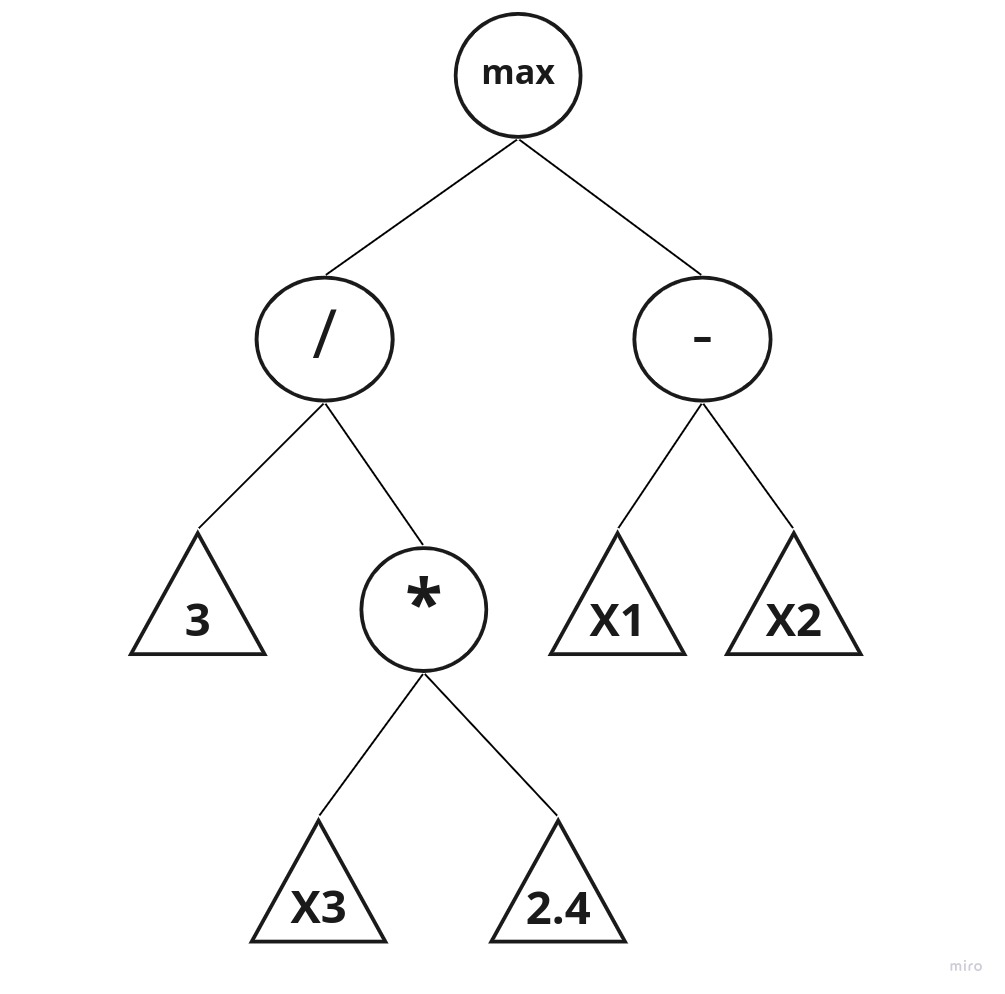
\includegraphics[width=0.4\textwidth]{../images/syntax_tree.jpg}
\end{center}
\caption{Početno stablo}
\label{fig:syntaxTree}
\end{figure}

\begin{figure}[!ht]
\begin{center}
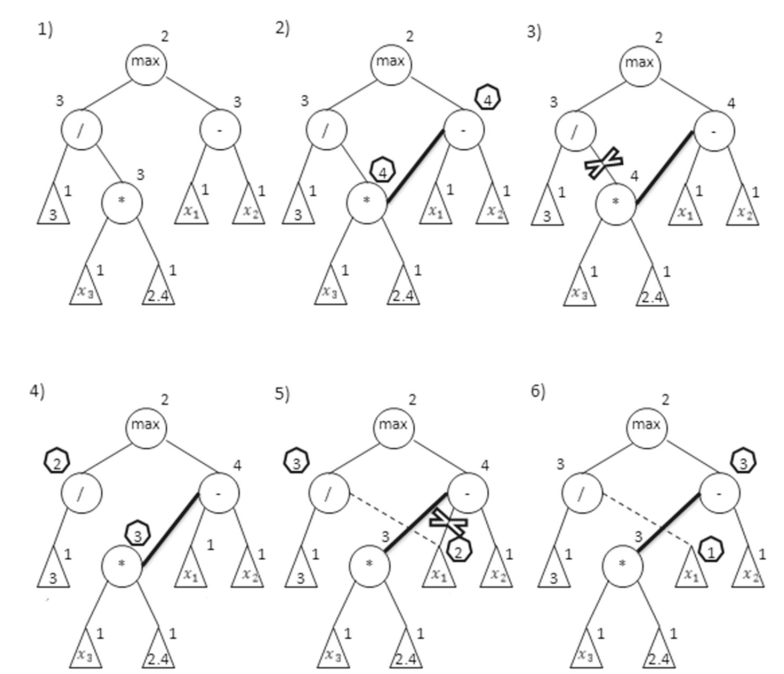
\includegraphics[width=0.95\textwidth]{../images/ett.png}
\end{center}
\caption{Primer primene ETT transformacija}
\label{fig:ett}
\end{figure}

Pomoću ETT je implementirana i lokalna pretraga koja koristi strategiju \textit{prvog poboljšanja}. Kada se naiđe na prvo stablo koje daje bolje rezultate na datom skupu podataka, ono se vraća kao trenutno najbolje rešenje iz čijeg susedstva će se dalje nastaviti pretraga. Kao funkcija na osnovu koje se poredi kvaliet stabala, uzet je koeficijent determinacije $R^{2}$. 


\subsection{Osnovni VNP algoritam}
\label{sec:basicVNP}

Uzimajući u obzir sve prethodno definisane pojmove, osnovna VNP procedura za simboličku regresiju se može predstaviti algoritmom \autoref{alg:BVNP}. 

\begin{algorithm}
\floatname{algorithm}{Algoritam}
\caption{Basic VNP(T, k_{max})}
\label{alg:BVNP}
  \begin{algorithmic}[1]
  \STATE \textbf{repeat}
    \STATE $k \leftarrow 1$ ;
    \WHILE {$k < k_{max}$}
        \STATE $T^{\prime} \leftarrow Shake(T, k)$;
        \STATE $T^{\prime}^{\prime} \leftarrow ETT(T^{\prime})$;
        \STATE $Neighborhood\_change(T, T^{\prime}^{\prime}, k)$;
    \ENDWHILE
    \STATE \textbf{until} nije ispunjen kriterijum zaustavljanja;
  \end{algorithmic}
\end{algorithm}

Kriterijum zaustavljanja osnovne VNP procedure može biti pronalazak tačnog rešenja, maksimalan dozvoljeni broj iteracija ili maksimalno vreme izvršavanja.

\end{document}